\section{Auswertung}

Fehler und Ausgleichsrechnungen werden mit dem Python-Paket ScyPy \cite{scypy} berechnet.

\subsection{Amplitudenmodulation mit Ringmodulator}

Mit dem Ringmodulator wird die Amplitude eines Signals moduliert. Das Eingans- und Ausgangssignal sind in \autoref{a} zu sehen. Das Trägersignal hatte eine Amplitude von $U_\text{T}=\SI{980}{\milli\volt}$ und die Frequenz $\omega_\text{T}=\SI{1}{\mega\hertz}$, das Modulationssignal hatte eine Amplitude von $U_\text{M}=\SI{116}{\milli\volt}$ und die Frequenz $\omega_\text{M}=\SI{50}{\kilo\hertz}$. Es entsteht eine Schwebung, die Trägerfrequenz ist hier nicht zu erkennen. Die prominentesten Linien in dem Frequenzspektrum in \autoref{b} sind die der Modulationsfrequenz. Dazwischen ist als kleinerer Peak auch die Trägerfrequenz zu sehen, die mit dem Ringmodulator nicht komplett unterdrückt wird, aber signifikant kleiner als die Seitenbänder ist.

\begin{figure}
	\centering
	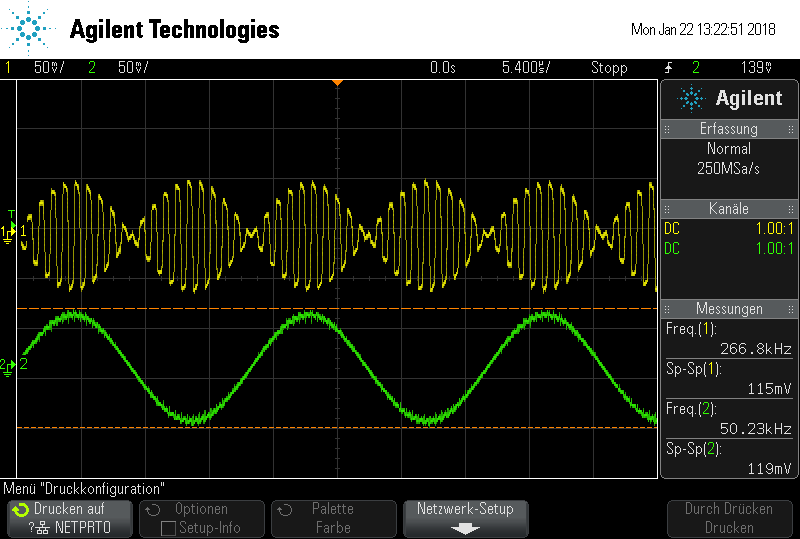
\includegraphics[width=\textwidth]{img/a_scope_230.png}
	\caption{Amplitudenmodulation - grün das Eingangssignal, gelb das amplitudenmodulierte Signal}
	\label{a}
\end{figure}

\begin{figure}
	\centering
	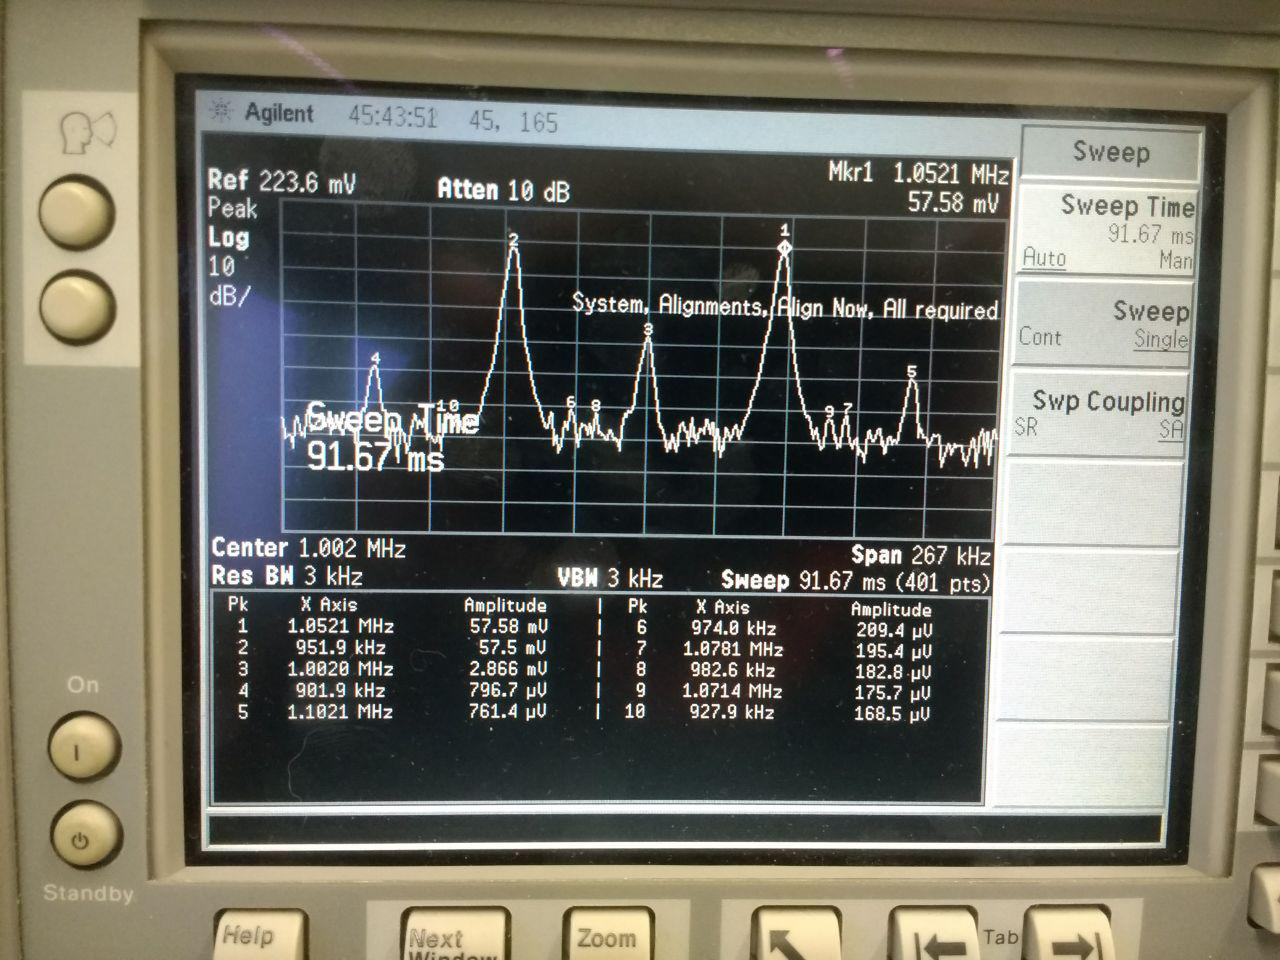
\includegraphics[width=\textwidth]{img/Aufgabenteil_b.jpg}
	\caption{Amplitudenmodulation - Peak 3 mit der Trägerfrequenz, Peak 1 und 2 die Seitenbänder}
	\label{b}
\end{figure}

\subsection{Amplitudenmodulation mit Trägerabstrahlung}

In \autoref{c1} ist das Fequenzspektrum einer amplitudenmodulierten Schwingung mit Trägerabstrahlung zu sehen. Das Trägersignal hatte eine Amplitude von $U_\text{T}=\SI{1.17}{\volt}$ und die Frequenz $\omega_\text{T}=\SI{1.55}{\mega\hertz}$, das Modulationssignal hatte eine Amplitude von $U_\text{M}=\SI{159}{\milli\volt}$ und die Frequenz $\omega_\text{M}=\SI{63}{\kilo\hertz}$. \autoref{c2} zeigt von dem gleichen Signal eine Oszilloskop-Aufnahme. In \autoref{c2} lässt sich der Modulationsgrad aus dem Verhältnis der Amplitude der Maxima und der Minima bestimmen. Da die Amplitude zwischen $U_\text{min} = U_\text{T}(1 - m)$ und $U_\text{max} = U_\text{T}(1 + m)$ schwankt, ist der Modulationsgrad
\[
	m =\frac{U_\text{max} - U_\text{min}}{U_\text{max} + U_\text{min}} = \frac{\SI{52}{\milli\volt} - \SI{26}{\milli\volt}}{\SI{52}{\milli\volt} + \SI{26}{\milli\volt}} = 0.33.
\]
Eine andere Methode, den Modulationsgrad zu bestimmen, ist mit der Pulshöhe der Träger- und Modulationsfrequenz im Frequenzanalysator. Dazu wird die Pulshöhe, die in der Einheit eines Leistungspegels angegeben wird, mit $P = 10^{L_P/10} \cdot \SI{1}{\watt}$ in eine Leistung umgerechet. Dann ist der Modulationsgrad $m = 4 \cdot \frac{P_\text{M}}{P_\text{T}}$
\[
	m_1 = 4 \cdot \frac{10^{-44.62/10}}{10^{-33.68/10}} = 0.322, \quad m_2 = 4 \cdot \frac{10^{-44.7/10}}{10^{-33.68/10}} = 0.316
\]

\begin{figure}
	\centering
	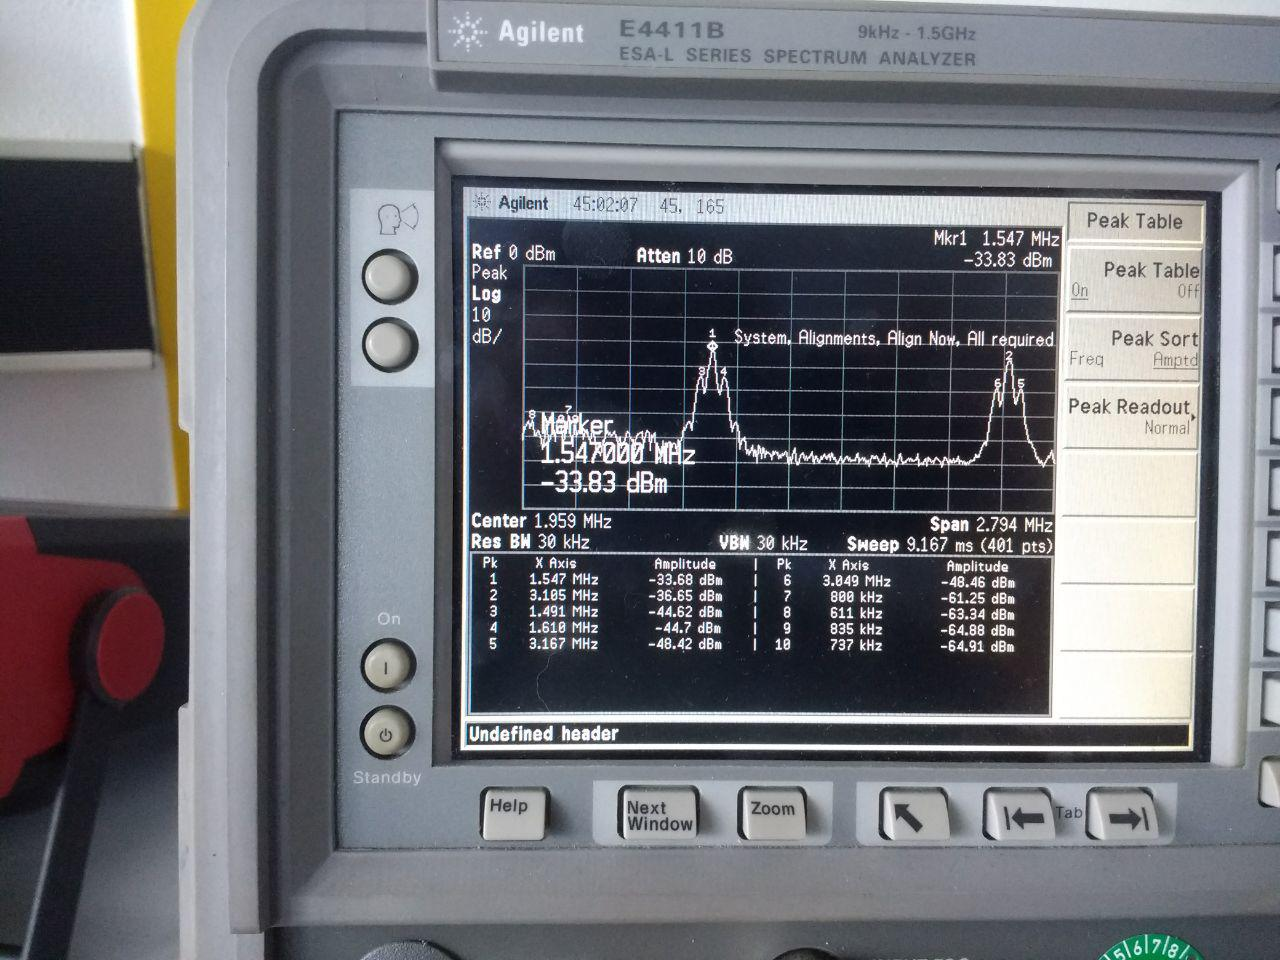
\includegraphics[width=\textwidth]{img/Aufgabenteil_c1.jpg}
	\caption{Amplitudenmodulation mit Oberwellen, Trägerabstrahlung und Seitenbändern}
	\label{c1}
\end{figure}

\begin{figure}
	\centering
	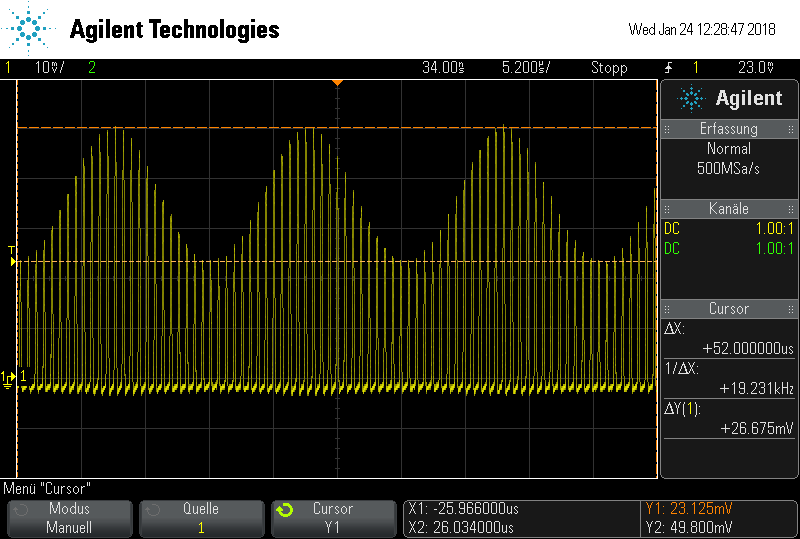
\includegraphics[width=\textwidth]{img/c_scope_247.png}
	\caption{Amplitudenmodulation - Bestimmung des Modulationsgrades}
	\label{c2}
\end{figure}

\subsection{Frequenzmodulation}

Das Trägersignal hatte eine Amplitude von $U_\text{T}=\SI{1.17}{\volt}$ und die Frequenz $\omega_\text{T}=\SI{1.55}{\mega\hertz}$, das Modulationssignal hatte eine Amplitude von $U_\text{M}=\SI{159}{\milli\volt}$ und die Frequenz $\omega_\text{M}=\SI{63}{\kilo\hertz}$. Die Breite der Verschmierung in \autoref{d1} ist an der maximalen Stelle $\Delta t = \SI{196}{\nano\second}$. Aus der Trägerfrequenz und der gemittelten Verschmierung ergibt sich eine Periodendauer von $T_\text{min} = \SI{645.2}{\nano\second} - \frac{\SI{196}{\nano\second}}{5} = \SI{606}{\nano\second}$ bzw. $T_\text{max} = \SI{645.2}{\nano\second} + \frac{\SI{196}{\nano\second}}{5} = \SI{684.4}{\nano\second}$.

\begin{figure}[t!]
	\centering
	\begin{subfigure}[t]{0.5\textwidth}
		\centering
		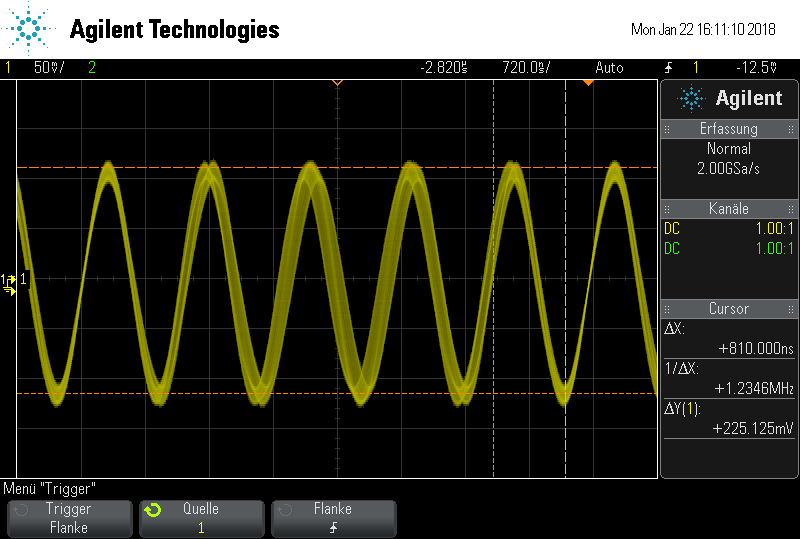
\includegraphics[width=\textwidth]{img/d_scope_233.png}
		\caption{Frequenzmodulation}
	\end{subfigure}%
	~
	\begin{subfigure}[t]{0.5\textwidth}
		\centering
		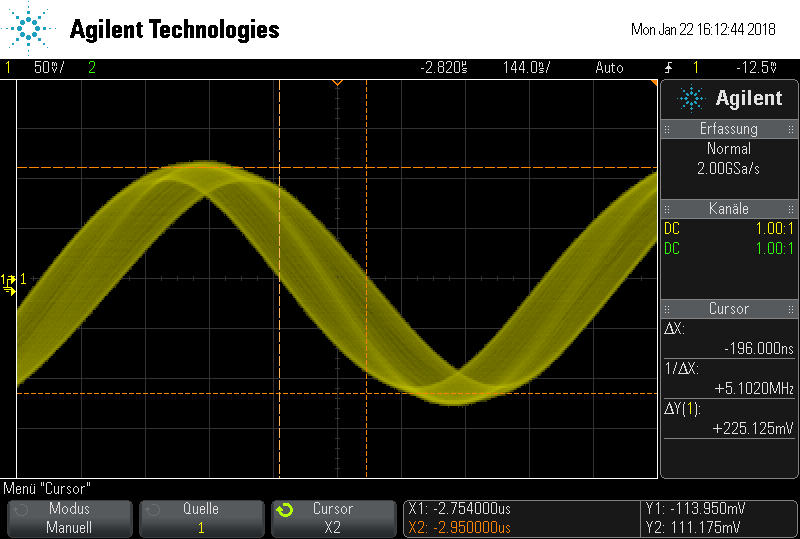
\includegraphics[width=\textwidth]{img/d_scope_234.png}
		\caption{Frequenzmodulation -- Detailansicht zur Bestimmung der Breite der Verschmierung}
	\end{subfigure}
	\caption{Frequenzmodulation eines sinusförmigen Trägersignals.}
	\label{d1}
\end{figure}

\begin{figure}
	\centering
	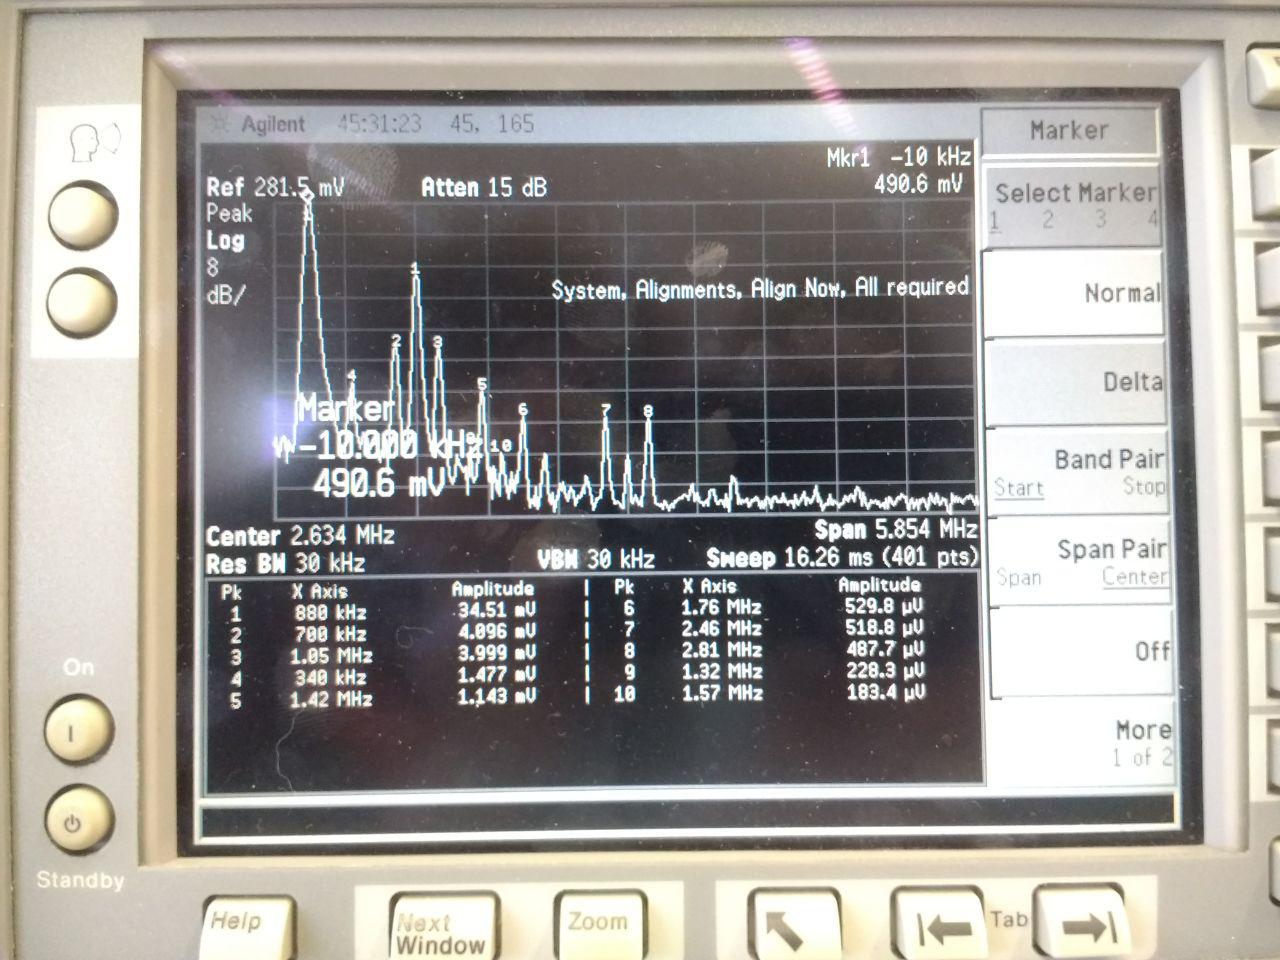
\includegraphics[width=\textwidth]{img/Aufgabenteil_d.jpg}
	\caption{Frequenzmodulation -- Frequenzspektrum}
	\label{d2}
\end{figure}

\subsection{Proportionalität zwischen Gleichspannung und Phase der Wechselspannung am Ringmodulator}

Die Annahme ist, dass eine Proportionalität zwischen Gleichspannung und Phase der Wechselspannung am Ringmodulator besteht. Um diesen Zusammenhang zu überprüfen, wird die Gleichspannung in Abhängikeit des Arguments des Cosinus gemessen. Es kann entweder die Laufzeit oder die Frequenz des Trägersignals variiert werden. In diesem Fall wird die Frequenz verändert, sodass

\begin{align}
\begin{split}
	U &= U_0 \cos(\omega_T \cdot t + \varphi)\\
	\arccos \frac{U}{U_0} &= \omega_T \cdot t + \varphi
\end{split}
\end{align}

gelten muss.

\begin{table}
\centering
\caption{Messwerte für den linearen Zusammenhang zwischen Gleichspannung und Phase der Wechselspannung.}
\begin{tabular}{ccc}
$\omega_T$/MHz &  $U$/mV &  $U_0$/mV \\
\midrule
         4.2 &  -138 &     496 \\
         4.4 &  -116 &     456 \\
         4.6 &   -86 &     400 \\
         4.8 &   -51 &     362 \\
         5.0 &   -16 &     348 \\
         5.2 &    20 &     388 \\
         5.4 &    52 &     446 \\
         5.6 &    89 &     488 \\
         5.8 &   116 &     509 \\
\end{tabular}
\label{tab:e}
\end{table}


Eine lineare Ausgleichsrechnung der Form $U/U_0 = A \cdot \omega_\text{T} + B$ an die Messwerte in \autoref{tab:e} ergibt die Parameter $A = -0.35 \pm 0.02$ und $B = 3.37 \pm 0.09$ und ist in \autoref{fig:e} dargestellt. Die geringen Fehler des linearen Fits von 5.7\% für die Steigung bzw. 2.8\% für den y-Achsenabschnitt zeigen, dass die Annahme eines ein linearen Zusammenhangs gerechtfertig ist.

\begin{figure}
	\centering
	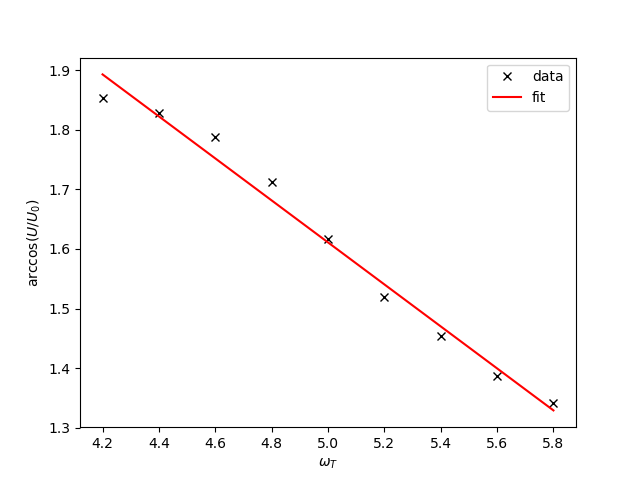
\includegraphics[width=\textwidth]{img/linear_fit.png}
	\caption{Lineare Ausgleichsrechnung zur Veranschaulichung des linearen Zusammenhangs zwischen $\cos\varphi$ und $U$.}
	\label{fig:e}
\end{figure}

\subsection{Demodulation einer amplitudenmodulierten Schwingung mit Ringmodulator}

In \autoref{f} ist die Oszilloskop-Aufnahme eines Signals zu sehen, dessen Amplitude zunächst moduliert und daraufhin wieder demoduliert wird. In gelb ist das Eingangssignal, die grüne Kurve ist das um einen festen Faktor phasenverschobene und in der Amplitude reduzierte Signal.

\begin{figure}
	\centering
	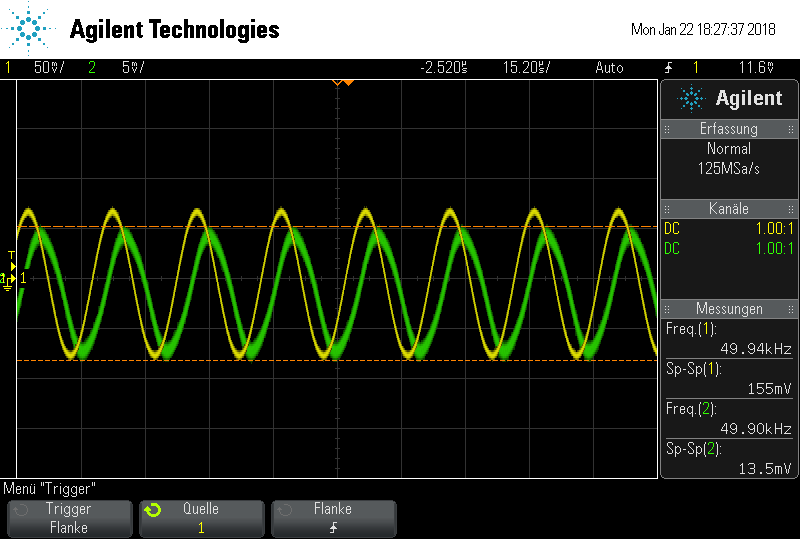
\includegraphics[width=\textwidth]{img/f_scope_235.png}
	\caption{Amplituden(de-)modulation - gelb das Eingangssignal, grün das amplitudenmodulierte und daraufhin demodulierte Signal}
	\label{f}
\end{figure}

\subsection{Demodulation mit Gleichrichterdiode}
\label{De-AM}

Die Diode in der Schaltung in \ref{blub} schneidet die negativen Halbwellen ab, wie in \autoref{nachDiode} zu sehen und das RC-Element filtert als Tiefpass die hohen Frequenzen aus dem Signal, dies ist in \autoref{nachRC} zu sehen. Wie zu erwarten ist die Amplitude des Ausgangsignal nach dem Tiefpass stark reduziert, die negativen Halbwellen sind nun aufgrund der Gleichrichterdiode positiv und das Ausgangssignal ist gegenüber dem Eingangssignal phasenverschoben.

\begin{figure}[t!]
	\centering
	\begin{subfigure}[t]{0.5\textwidth}
		\centering
		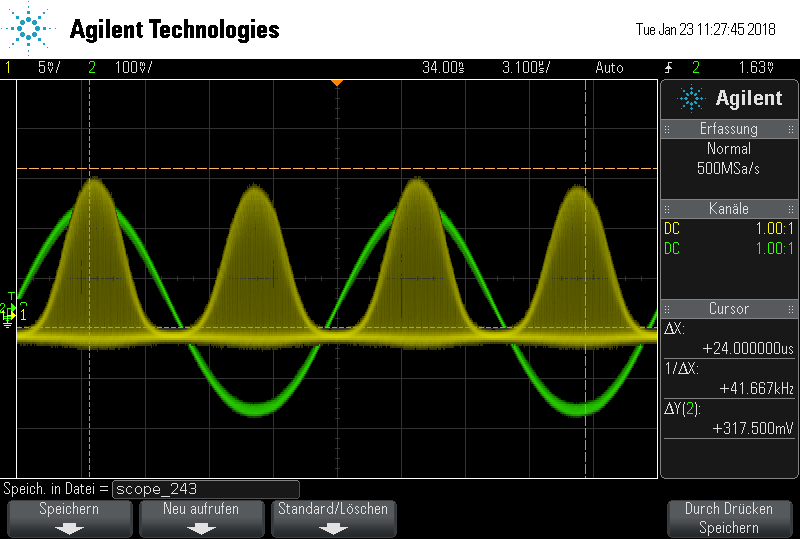
\includegraphics[width=\textwidth]{img/g_scope_243.png}
		\caption{Das Eingangssignal ist in grün abgebildet, in gelb das Signal nach der Diode in der Schaltung in \autoref{blub}.}
		\label{nachDiode}
	\end{subfigure}%
	~
	\begin{subfigure}[t]{0.5\textwidth}
		\centering
		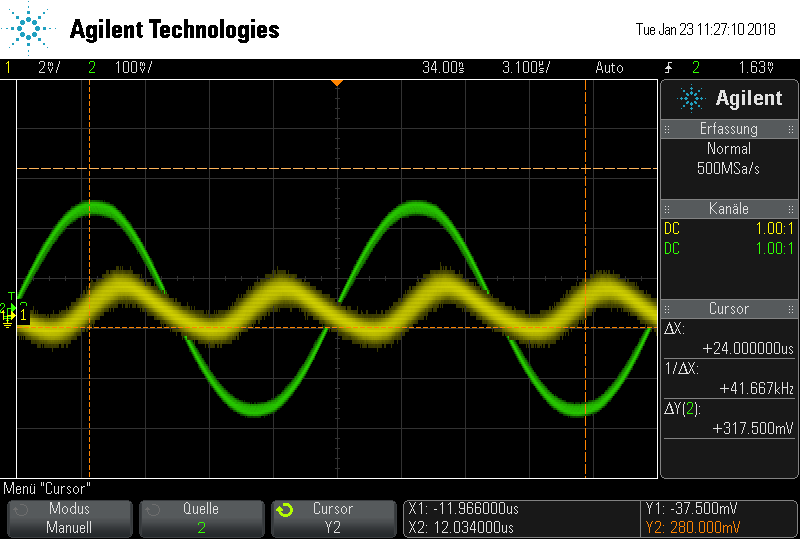
\includegraphics[width=\textwidth]{img/g_scope_242.png}
		\caption{Das Einganssignal ist wieder in grün, in gelb das demodulierte Ausgangssignal nach dem Tiefpass.}
		\label{nachRC}
	\end{subfigure}
	\caption{Demodulation eines amplitudenmodulierten Signals mit einer Gleichrichterdiode.}
\end{figure}

\subsection{Demodulation einer frequenzmodulierten Schwingung}

In \autoref{amp} ist mit der Schaltung in \autoref{blub} aus dem frequenzmodulierten Signal eine Amplitudenmodulation gemacht worden. \autoref{De-FM} und \autoref{De-FM-RC} zeigen die anschließende Demodulation mit einer Gleichrichterdiode und einem RC-Tiefpass wie bereits in \autoref{De-AM} durchgeführt.

\begin{figure}[t!]
	\centering
	\begin{subfigure}[t]{0.5\textwidth}
		\centering
		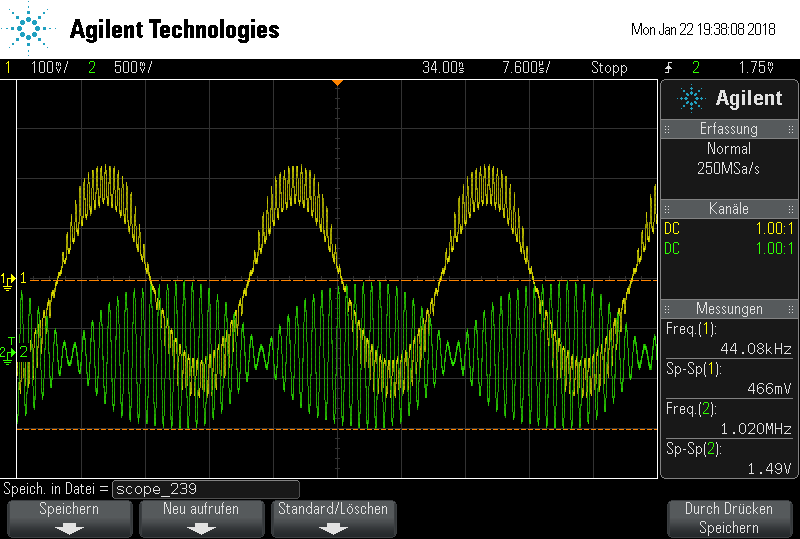
\includegraphics[width=\textwidth]{img/h_scope_239.png}
		\caption{In gelb ist das Eingangssignal gezeigt, in grün das modulierte Signal -- durch den LC-Kreis wird aus der frequenzmodierten Spannung ein amplitudenmoduliertes Signal.}
		\label{amp}
	\end{subfigure}%
	~
	\begin{subfigure}[t]{0.5\textwidth}
		\centering
		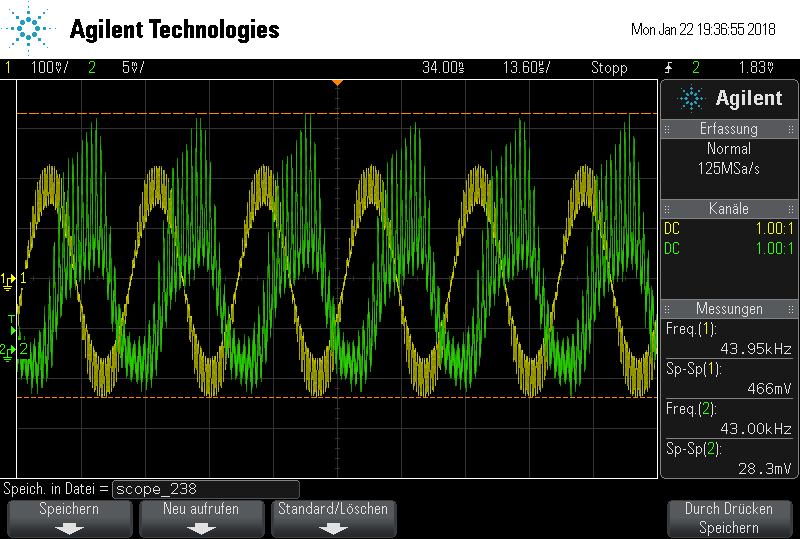
\includegraphics[width=\textwidth]{img/h_scope_238.png}
		\caption{Mit einer Gleichrichterdiode werden die negativen Halbwellen abgeschnitten.}
		\label{De-FM}
	\end{subfigure}
	\\
	\begin{subfigure}[t]{0.5\textwidth}
		\centering
		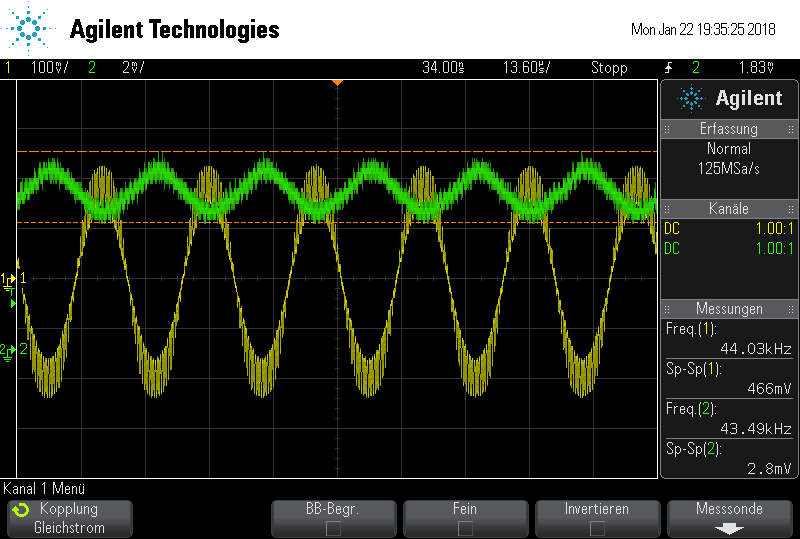
\includegraphics[width=\textwidth]{img/h_scope_237.png}
		\caption{Das in grün dargestellte Signal ist demoduliert und wurde nach dem Tiefpass abgegriffen.}
		\label{De-FM-RC}
	\end{subfigure}
	\caption{Demodulation einer frequenzmodulierten Schwingung.}
\end{figure}

\FloatBarrier
